\documentclass[aspectratio=169]{beamer} % O parâmetro aspectratio com valar 16:9 deixa o slide em widescreen

\usepackage[brazil]{babel}
\usepackage[utf8]{inputenc}
\usepackage[T1]{fontenc}

\usetheme{Madrid}
\setbeamertemplate{navigation symbols}{}

\title[Educação em Tecnologias Digitais]{Educação em Tecnologias Digitais}

\author[Diego S. C. Nascimento]{Diego Silveira Costa Nascimento}

\institute[IFRN]{
Instituto Federal de Educação, Ciência e Tecnologia do Rio Grande do Norte\\
diego.nascimento@ifrn.edu.br
}

\date[\today]{\today}

\begin{document}

\begin{frame}[plain]
	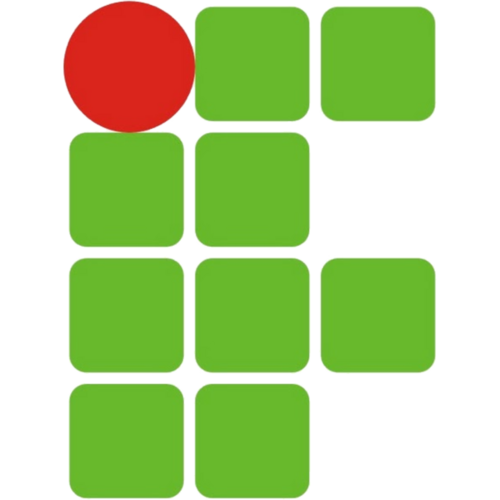
\includegraphics[scale=0.2]{img/IFRN}
	\titlepage
\end{frame}

\logo{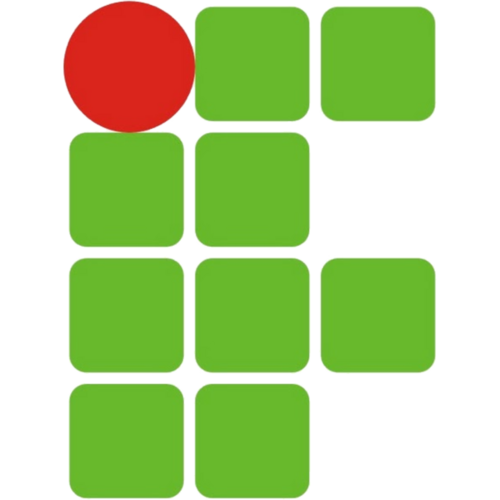
\includegraphics[scale=0.1]{img/IFRN}}

\begin{frame}
	\frametitle{Ementa do Curso}
  	\tableofcontents
\end{frame}

\AtBeginSection[]{
	\begin{frame}
		\frametitle{Ementa}
		\tableofcontents[currentsection]
	\end{frame}
}

\section{Sistemas Operacionais}

\begin{frame}
	\frametitle{O que é um sistema operacional (SO)?}
	
	\begin{block}{Definição}
		
	\end{block}
\end{frame}

\section{Internet}

\section{Inteligência Artificial na Educação}

\section{Editor de Texto}

\section{Editor de Apresentação}

\section{Editor de Planilha Eletrônica}

\end{document}